\documentclass[../main.tex]{subfiles}
\graphicspath{{\subfix{../Figures/}}}
\begin{document}

    \begin{frame}{Definitions} 
        \begin{itemize}
            \item A graph $G=(V,E)$ is a collection of $n$ vertices and $m$ edges.
            \item A hypergraph $H=(V,E)$ is a generalization of a graph to capture higher order relations between vertices.
            \item An interesting property of a graph is its conductance $\phi$: 
	            \begin{columns}
	            	\column{0.4\textwidth}
	            	\begin{block}{Conductance}
	            		$\phi(S) = \frac{E(S, \bar{S})}{\min(\text{vol}(S), \text{vol}(\bar{S}))}$
	            	\end{block}
	            \end{columns}
            It measures how well inter-connected the cut $S$ is, and well separated from the rest of the graph.
            \item In the Local Clustering problem, you want to find a cut $(S, \bar{S}) : S\subseteq V \land S\cup \bar{S}=V$ around a vertex $v\in S$ such that the conductance is at most a parameter $\hat{\phi}$.
            \item The way to find good clusters is by studying mixing and leaking properties of random walks in a graph. 
        \end{itemize}
    \end{frame}
    
    \begin{frame}{Random Walks in graphs}
        Local clustering in graphs is often achieved by random walks. Here are some useful definitions:
        \begin{itemize}
            \item Random walks are \textit{lazy} (w.p. $\frac{1}{2}$ you do not move)
            
            \begin{columns}
                \column{0.8\textwidth}
                \begin{block}{Transition probability matrix}
                    $M = \frac{1}{2}(I + AD^{-1})$ 
                \end{block}
                \begin{block}{Evolution of probability vector}
                    $\bold{p}_{t+1} = M \bold{p}_t$
                \end{block}
            \end{columns}
            \item The Laplacian matrix $\mathcal{L}=I - AD^{-1}$ describes the rate of convergence of the probability vector wrt the time:
            \begin{columns}
                \column{0.4\textwidth}
                \begin{block}{Derivative of $p_t$ wrt time}
                    $\frac{d \bold{p}_t}{d t} = - \mathcal{L} \bold{p_t}$
                \end{block}
            \end{columns}
        \end{itemize}
    \end{frame}
    
    
    \begin{frame}{Random Walks in graphs}
        \begin{itemize}
            \item Random walks converge to the stationary distribution $\pi(u) = \frac{d(u)}{\text{vol}(G)}$
                \begin{columns}
                    \column{0.6\textwidth}
                    \begin{block}{Convergence to stationary distribution}
                        when $t\to\infty \implies \bold{p}_t\to \pi$
                    \end{block}
                \end{columns}
            \item Studying how fast the probability vector converges to stationary distribution is called \textit{mixing}, and it is done with the Lovasz-Simonovits curve \cite{Lovsz1993RandomWI}.
        \end{itemize}
        
    \end{frame}
    
    \begin{frame}{Lovasz-Simonovits curve}
            It is easy to define the Lovasz Simonovits curve using sweep cuts:
                \begin{columns}
                    \column{0.8\textwidth}
                    \begin{block}{Sweep Cut}
                        $S_j(\bold{p}_t) = \{u\in V: \frac{p_t(u)}{d(u)} \text{ is maximized} \land |S_j(\bold{p}_t)| = j\}$
                    \end{block}
                \end{columns}
            \begin{columns}
            	\column{0.6\textwidth}
    	        \begin{itemize}
	            \item LS curve: for $k = \text{vol}(S_j(\bold{p}_t))$ for some $j\in[0,n]$
	                \begin{columns}
	                    \column{1\textwidth}
	                    \begin{block}{Lovasz-Simonovits curve}
	                        $I_t(k) = \sum_{u\in S_j(\bold{p}_t)} p_t(u)$
	                    \end{block}
	                \end{columns}
	            \item Properties: concave, it decreases until it converges to a straight line:
	                \begin{columns}
	                    \column{1.\textwidth}
	                    \begin{block}{Lovasz-Simonovits curve is decreasing} 
	                        $I_{t+1}(k) \leq I_{t}(k)$
	                    \end{block}
	                \end{columns}
		        \end{itemize}
	        \column{0.4\textwidth}
	        \raisebox{.0\height}{
	        	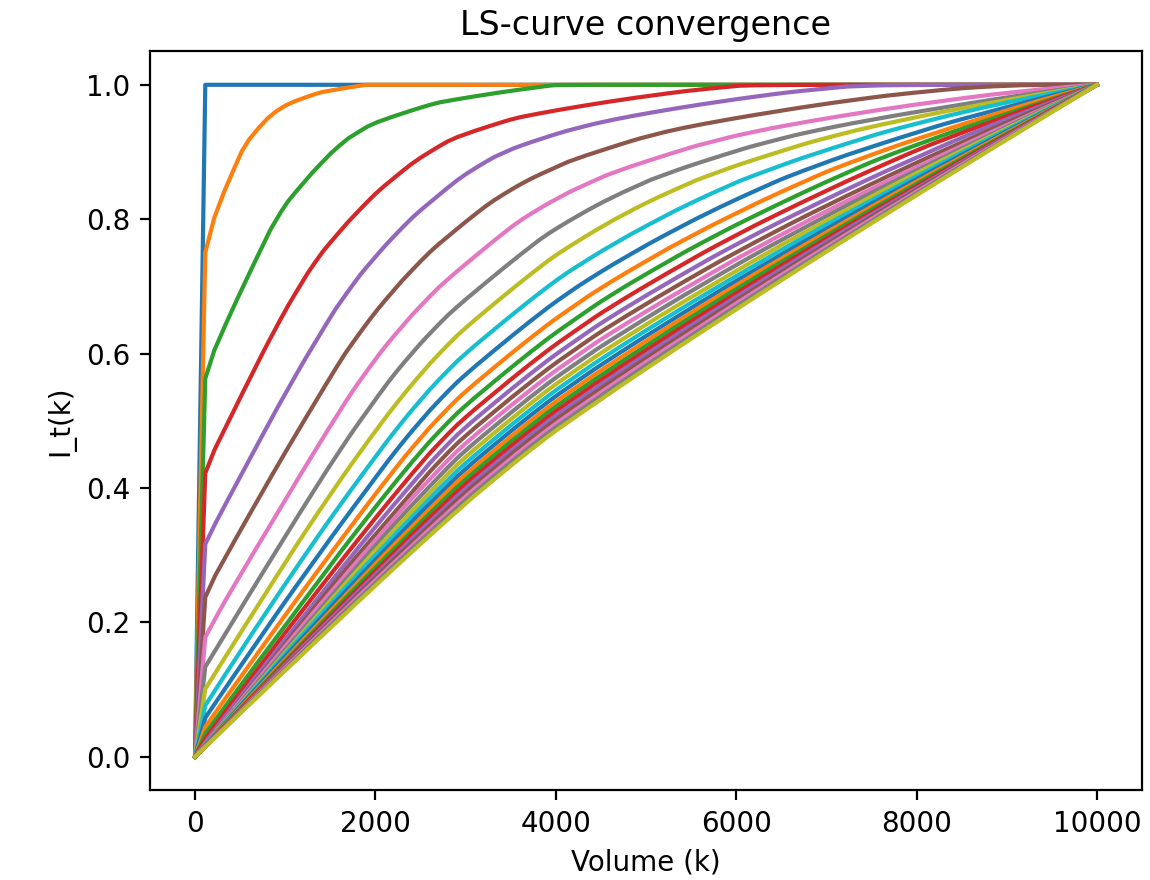
\includegraphics[width=0.9\textwidth]{LS-curve_convergence}
        	}
    	\end{columns}
    \end{frame}
    
    \begin{frame}{1. Studying mixing with Lovasz-Simonovits curve}
        \begin{itemize}
            \item It is possible to study the mixing time of a random walk by studying how fast the LS curve converges to a straight line. In particular, in between time steps, the LS-curve decreases piece-wise to be below a \textit{large} chord depending on the conductance $\hat{\phi} = \min_{j\in[1,n], t}\phi(S_j(\bold{p}_t))$: $\forall k\in[0,\text{vol}(G)]$, and $\hat{k}:=\min(k, \text{vol}(G)-k)$
                \begin{columns}
                    \column{0.5\textwidth}
                    \begin{block}{Recursive upper bound of LS curve}
                        $I_{t+1}(k) \leq \frac{1}{2}(I_t(k-\hat{\phi} \hat{k}) + I_t(k+\hat{\phi} \hat{k}))$
                    \end{block}
                	\column{0.5\textwidth}
                	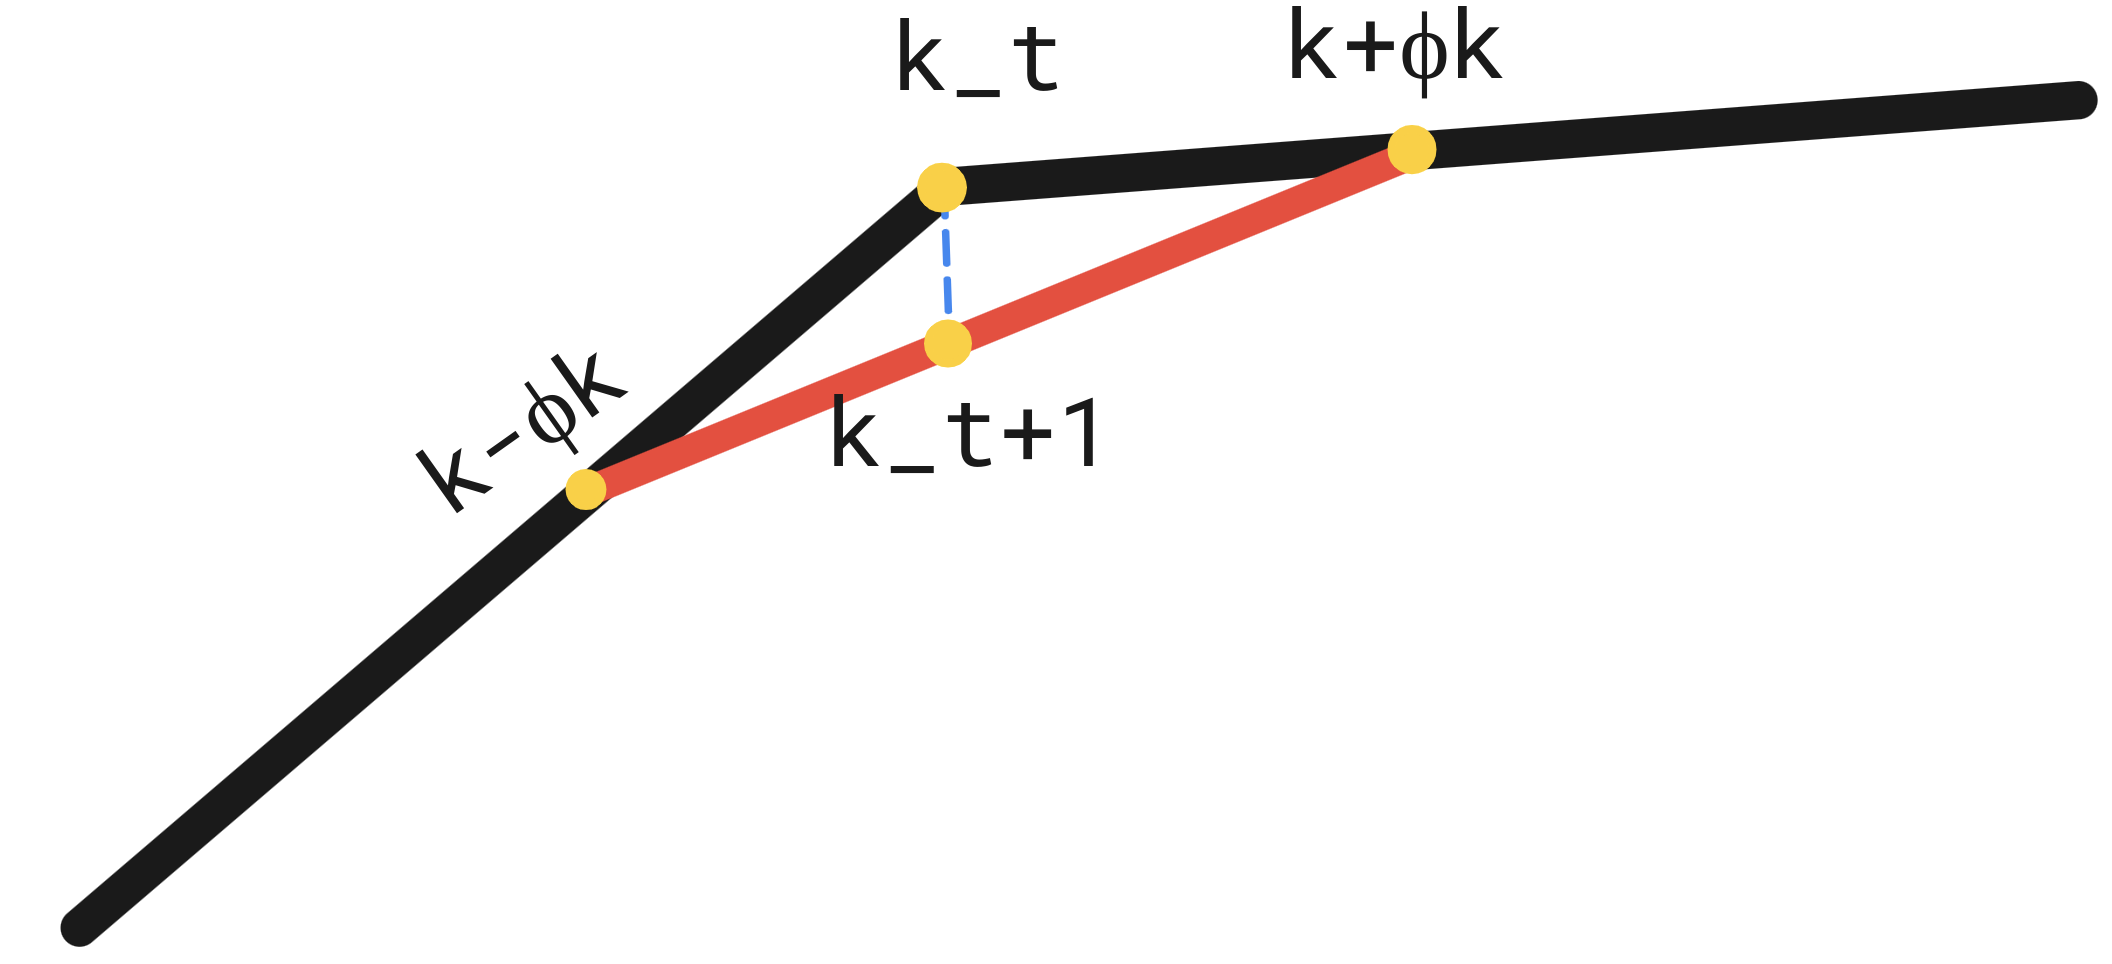
\includegraphics[width=1.\textwidth]{ls_recursive_upper_bound}
                \end{columns}
           \item This allows for exponentially fast convergence:
                \begin{columns}
                    \column{0.6\textwidth}
                    \begin{block}{Exponentially fast mixing wrt time}
                        $I_{t}(k) - \pi(S_j(\bold{p}_t)) \leq \sqrt{\hat{k}}e^{-t \hat{\phi}^2}$
                    \end{block}
                \end{columns}
        \end{itemize}
    \end{frame}
    
    \begin{frame}{2. Leaking of random walks in a graph}
        \begin{itemize}
            \item Leaking is the opposite of mixing: it provides a lower bound on the mixing time of a random walk, based on the optimal conductance of the graph.
            \item For graphs, leaking is very simple: when $p_0= \psi_S$ for some $S\subseteq V$, then
                \begin{columns}
                    \column{0.7\textwidth}
                    \begin{block}{Leaking wrt optimal conductance $\phi^*$}
                        $p_t(S) \geq 1 - t\phi(S)$
                    \end{block}
                \end{columns}
            \item To conclude, it can also be proved that the volume of $S^g$ s.t. $\forall v\in S^g\subseteq S$ when $p_0 = \chi_v$ then $p_t(S)\geq 1-t\phi^*(S)$ is large:
                \begin{columns}
                    \column{0.7\textwidth}
                    \begin{block}{Volume of $S^g$ is large}
                        $\text{vol}(S^g) \geq \frac{1}{2}\text{vol}(S)$
                    \end{block}
                \end{columns}
        \end{itemize}
    \end{frame}
    
    \begin{frame}{Mixing+leaking = clustering algorithm}
        \begin{itemize}
            \item Assumption: there is a set $S$ of large volume (but $\leq \frac{1}{2}\text{vol}(G)$), s.t. for a parameter $\hat{\phi}$, its conductance is $\phi(S) \leq \frac{\hat{\phi}^2}{\log(n)} = \phi^*$
            \item You pick a vertex $v$ at random according to the stationary distribution (with good probability it falls in $S^g$) and evolve the probability vector from $\bold{p}_0 = \chi_v$ for $t=\frac{1}{4\phi^*}$ iterations.
            \item By leaking: $p_t(S) - \pi(S) \geq 1 - t\phi^* - \frac{1}{2} \geq \frac{1}{4}$
            \item in contrast, by mixing $p_t(S) - \pi(S) \leq \sqrt{\text{vol}(S)}e^{-t\hat{\phi}^2}$
            \item This allows to conclude that $\hat{\phi} \leq \sqrt{\log(n) \phi^*}$ \textit{not too far} from the original conductance \cite{SpielmanClustering}.
        \end{itemize}
    \end{frame}
    
    \begin{frame}{Local clustering algorithm for hypergraphs}
        \begin{itemize}
            \item In order to find a proper clustering algorithm for hypergraphs, we need to generalize both mixing and leaking results to hypergraphs. 
            \item Mixing: there have attempts to prove mixing using continuous diffusion processes \cite{Takai_2020}.
            \item Leaking: no known leaking result as far as we know.
        \end{itemize}
    \end{frame}
\end{document}